\documentclass{beamer}

% Packages

% Sets

% Formal statements


\title{Diseño y análisis de algoritmos \\ ISIS1105}
\author{Daniel R. Barrero R.}
\institute{Universidad de los Andes}

\begin{document}
\frame{\titlepage}

\begin{frame}{LHRRs}
	\begin{thm}[1]\label{thmhr}
		The initial value problem
		\begin{displaymath}
			\begin{cases}
				t(0)= v_0,\ t(1)= v_1,\cdots t(k-1)= v_{k-1}\\
				t(n)= a_1t(n-1) + \cdots + a_{k-1}t(n-k+1) + a_kt(n-k)
			\end{cases}
		\end{displaymath}
		has a unique solution
		\begin{equation*}
			t(n) = c_0\alpha_0^n + c_1\alpha_1^n + \cdots + c_{k-1}\alpha_{k-1}^n
		\end{equation*}
		where the $c_i$ are complex numbers and the $\alpha_i$ are the roots of
		the lhrr, provided these numbers are distinct.
	\end{thm}
\end{frame}

%

%% Inhomogeneous linear
\begin{frame}{The towers of Hanoi}
	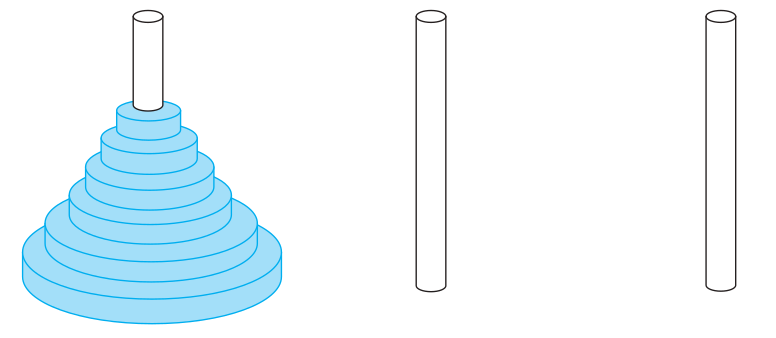
\includegraphics[width=0.5\textwidth]{hanoi.png}

	\begin{itemize}
		\item[]
		\item Poner los discos en orden de tamaño en la segunda clavija,
			moviendo un disco a la vez.
		\item No se puede poner un disco más grande sobre uno más pequeño.
	\end{itemize}
\end{frame}

%

\begin{frame}{The towers of Hanoi}
	\lstinputlisting[language=Java, firstline=2, lastline=17]{Aula04.java}
\end{frame}

%

\begin{frame}{LRRs - The towers of Hanoi}
	The associated initial value problem is
	\begin{displaymath}
		\begin{cases}
			t(0)= 0\\
			t(m)= 2t(m-1) + 1,\ m \geq 1.
		\end{cases}
	\end{displaymath}
	and its recurrence relation is \emph{not} homogeneous.
	\begin{defn}
		A \emph{linear recurrence relation (lrr)} is of the form
		\begin{equation}\label{lrr}
			t(n) + b_1t(n-1) + \cdots + b_{k-1}t(n-k+1) + b_kt(n-k)= q.
		\end{equation}
		When $q \neq 0$, it is called the \emph{inhomogeneous part} of \eqref{lrr}.
		The \emph{characteristic equation} of \eqref{lrr} is the characteristic
		equation of $t(n) + \sum_{i= 1}^k b_it(n-i)= 0$, which is the
		\emph{homogeneous part} of \eqref{lrr}.
	\end{defn}
\end{frame}

%

\begin{frame}{LRRs - The towers of Hanoi}
	If $t(n) - 2t(n-1) = 1$ for all $n \geq 1$, then $t(n-1) - 2t(n-2) = 1$ for
	all $n \geq 2$. Therefore, the Hanoi problem can be reformulated as

	\begin{displaymath}
		\begin{cases}
			t(0)= 0,\ t(1)= 1\\
			t(n)= 3t(n-1) - 2t(n-2),\ n \geq 2.
		\end{cases}
	\end{displaymath}
	Thanks to theorem \ref{thmhr}, its solution is of the form
	\begin{equation*}
		t(n) = c_02^n + c_11^n,
	\end{equation*}
	where the constants $c_0$ and $c_1$ can be found by solving the linear
	system
	\begin{displaymath}
		\begin{cases}
			c_0 + c_1 = 0\\
			2c_0 + c_1 = 1.
		\end{cases}
	\end{displaymath}
\end{frame}

%

\begin{frame}{LRRs - Replace inhomogeneous with homogeneous}
	We solved the inhomogeneous Hanoi problem by making it a particular case
	of a higher-degree homogeneous problem. This applies in general for the
	following family of problems.
	\begin{thm}[2]\label{ht}
		If the initial value problem
		\begin{displaymath}(4)
			\begin{cases}
				t(0)= v_0, \cdots, t(k-1)= v_{k-1}\\
				t(n) + \sum_{i= 1}^k b_it(n-i)= q,\ n \geq k
			\end{cases}
		\end{displaymath}
		is such that $q = c^np(n)$, where $c$ is a positive constant and
		$p(n)$ is a polynomial of degree $d$, then it is equivalent to a
		homogeneous problem of degree $k+d+1$ with characteristic equation
		\begin{equation*}
			E(x)(x-c)^{d+1} = 0
		\end{equation*}
		where $E(x) = 0$ is the characteristic equation of the recurrence
		in (4).
	\end{thm}
\end{frame}

%

\begin{frame}{LRRs - homogenization trick}
	We see that theorem \ref{ht} allows us to replace an inhomogeneous problem
	with a homogeneous one. Its application will be called the
	\emph{homogenization trick}.
\end{frame}

%% Divide and conquer
\begin{frame}{Divide and conquer}
	Consider the merge sorting algorithm
	\lstinputlisting[language=Java, firstline=28, lastline=49]{Aula04.java}
\end{frame}

%

\begin{frame}{Divide and conquer}
	Its time complexity satisfies the initial value problem
	\begin{displaymath}
		\begin{cases}
			t(1)= 1\\
			t(n)= t\left( \lceil n/2 \rceil \right) +
			t\left( \lfloor n/2 \rfloor \right) + cn,\ n \geq 2
		\end{cases}
	\end{displaymath}
	where $cn$ is the time complexity of the \texttt{merge} subroutine.
	If $n$ is even, the recurrence becomes
	\[
		t(n)= 2t(n/2) + cn.
	\]
\end{frame}

%

\begin{frame}{D \& C - merge sort}
	\textbf{Change of variable.} Let $n= 2^m$ and let $T(m)= t(2^m)$.
	The initial value problem becomes
	\[
		\begin{cases}
			T(0)= 1\\
			T(m)= 2T(m-1) + c2^m,\ m > 0.
		\end{cases}
	\]
	Let us apply the homogenization trick.

	\bigskip
	For $m > 1$ we have $T(m-1) = 2T(m-2) + c2^{m-1}$. Multiplying by 2 on
	both sides gives
	\[
		2T(m-1) = 4T(m-2) + c2^m,\ m > 1.
	\]
	Then for $m > 1$
	\[
		\begin{cases}
			T(m) - 2T(m-1) = c2^m\\
			2T(m-1) - 4T(m-2) = c2^m.
		\end{cases}
	\]
\end{frame}

%

\begin{frame}{D \& C - merge sort}
	Subtracting the two equations and computing $T(1)$, we obtain the homogeneous
	initial value problem
	\[
		\begin{cases}
			T(0)= 1,\ T(1)= 2 + 2c\\
			T(m) - 4T(m-1) + 4T(m-2)= 0,\ m > 1.
		\end{cases}
	\]
	We obtain $T(m) = 2^m + cm2^m$. Since $m = \log n$, we conclude
	$t(n) = n + cn\log n$, which is in $O(n\log n)$.

	\begin{qtn}
		How can one conclude $t(n) \in O(n\log n)$ for all $n$ and not
		just for powers of two?
	\end{qtn}
\end{frame}

%

\begin{frame}{D \& C - fast exponentiation}
	Consider the following algorithm
	
	\lstinputlisting[language=Java, firstline=89, lastline=98]{Aula04.java}

	Let $t(n)$ denote the number of multiplications \texttt{'*'}. It defines the
	initial value problem
	\[
		\begin{cases}
			t(0)= 0\\
			t(n)= t(n/2) + 1,\ n > 0\ \text{even}\\
			t(n)= t(n-1) + 1,\ n > 0\ \text{odd}.
		\end{cases}
	\]
\end{frame}
\end{document}
